\documentclass[noback,portrait,twocolumn]{cuposter}
\usepackage{amsmath}
\usepackage{amsfonts}
\usepackage{psfrag}
\usepackage{helvet}
\usepackage{wrapfig}
\usepackage{tabularx,multirow,multicol}
\usepackage{algorithm}
\usepackage{algpseudocode}

%\def\E{\mbox{{\rm E}}}

\begin{document}

% general
\definecolor{Red}{rgb}{1.0,0.2,0.2}
\definecolor{DarkRed}{rgb}{0.6,0.0,0.0}
\definecolor{DarkGreen}{rgb}{0.0,0.4,0.0}
%\definecolor{DarkBlue}{rgb}{0.0,0.0,0.4}
\definecolor{DarkBlue}{rgb}{.08,.46,0.77}
%\definecolor{Blue}{rgb}{.2,.2,1.0}
\definecolor{Blue}{rgb}{.08,.46,0.77}
\definecolor{Purple}{rgb}{0.7,0.1,0.7}
\definecolor{LightGray}{gray}{0.75}
\definecolor{Yellow}{rgb}{0.8,0.8,0.1}

\definecolor{BrightRed}{rgb}{0.95,0.0,0.0}
\definecolor{BrightGreen}{rgb}{0,0.8,0}
\definecolor{BoundaryColor}{named}{Blue}
\definecolor{EmphasisColor}{rgb}{1,0,0.2}


%style
\def\bordercolor{BoundaryColor}
\def\sectionheadcolor{BrightRed}
\def\colsepcolor{BoundaryColor}

\renewcommand{\ItemizeColour}{\color{DarkRed}}


% Definitions.
% --------------------
\newcommand{\clb}[1]{{\color{Red} \bf #1}}

\title{ReFr: An Open-Source \\
Reranker Framework}
\author{Daniel M. Bikel, Keith B. Hall}  
\email{\{dbikel,kbhall\}@google.com}
\address{Google Inc.}

\setlength{\SpaceBeforeText}{-2cm}

\makeposter

\renewcommand{\SectionColour}{\color{Blue}}
\section{Introduction}
\begin{itemize}
\item ReFr grew out of 2011 CLSP summer workshop at Johns Hopkins: \\
      Generating Confusions for Discriminative Language Modeling
  \begin{itemize}
  \item automatic generation of confusions from text scales to arbitrary size
  \item needed software that was both flexible and scalable
  \end{itemize}
\item Reranker Framework (ReFr) has the following properties
  \begin{itemize}
    \item industrial strength
    \item academic flexibility: features and learning methods
    \item flexible design: dynamic object composition
  \end{itemize}
\end{itemize}

\section{Data Format for I/O}
\begin{itemize}
\item Problem: rescoring native formats of a baseline system (lattices
  for ASR; hypergraphs for MT)
  \begin{itemize}
    \item limits scope of features and
    \item makes it difficult to run external text processors
  \end{itemize}
\item ReFr
  \begin{itemize}
  \item does k-best rescoring for maximum flexibility
  \item uses Google Protocol Buffers \cite{protobuf} as native I/O format
  \item provides tools to convert other formats to native format
  \end{itemize}
\end{itemize}

\nobreak
\section{Core Learning Framework}
\begin{minipage}[t]{23.5cm}{
% redefine \ForAll so it comes out as "foreach"
\renewcommand\algorithmicforall{\textbf{foreach}}
\begin{algorithmic}
\Procedure{Train}{$T~=~\{e_1, \ldots, e_n\},
                   D~=~\{d_1,\ldots,d_m\}$}
  \While{\Call{NeedToKeepTraining}{}()}
    \State \Call{TrainOneEpoch}{$T$}
    \State \Call{Evaluate}{$D$}
  \EndWhile
\EndProcedure
\State
\Procedure{TrainOneEpoch}{$T$}
  \ForAll{training example $e_i$}
    \State \Call{ScoreCandidates}{$e_i$}
    \If {\Call{NeedToUpdate}{}()}
      \State \Call{Update}{}()
    \EndIf
  \EndFor
\EndProcedure
\State
\Procedure{ScoreCandidates}{$e_i$}
  \ForAll{candidate hypothesis $c_j \in e_i$}
    \State $c_j.\texttt{score} \leftarrow K(w_t, c_j)$
  \EndFor
\EndProcedure
\end{algorithmic}
}\end{minipage}
\begin{minipage}[t]{10cm}{
\vspace{1cm}
  \begin{itemize}
  \item $e_{i}=\{c_{1},\ldots,c_{k}\}$ is a \emph{training example},
        each $c_{j}$ is a \emph{candidate hypothesis}.
  \item $d_{i}=\left\{ c_{1},\ldots,c_{k}\right\} $ is a held-out development data        example
  \item $\mathcal{K}$ is a \emph{kernel function}.
  \end{itemize}
}\end{minipage}

\subsection{Choose your update}
\begin{itemize}
  \item Basic perceptron update: \[
        w_{t+1}=w_{t}+R_{t}\left[\Phi\left(y_{\mathrm{oracle}}\left(e_{i}\right)\right)-\Phi\left(\hat{y}\left(e_{i}\right)\right)\right] \]
        where $\Phi$ maps input into a \textit{feature space}, $\mathbb{R}^{N}$
        and $R_t$ is a \textit{learning rate}.
  \item Many learning variants can be expressed simply as differing ways of choosing $\Phi$, $R_t$, $y_{\mathrm{oracle}}$ and $\hat{y}$
  \item ReFr makes it easy to define and alter $\Phi$, $R_t$, $y_{\mathrm{oracle}}$ and $\hat{y}$ and the entire \textsc{Update()} method (e.g., \cite{hazan2010direct,crammer2003ultraconservative})
\end{itemize}

\subsection{...at run-time}

\begin{itemize}
  \item ReFr contains a lightweight yet powerful \textit{\textbf{interpreted language}}
  \item Language very similar to subset of C++ used for constructors
  \item Can define primitives, Factory-constructible objects and vectors
  \item Can define objects that wrap other objects
\end{itemize}

\columnbreak

\subsubsection{Example configuration}
\small
\begin{verbatim}
model_file = "my_model_file";  // model output file
model =
  PerceptronModel(name("my model"),
                  score_comparator(DirectLossScoreComparator()));
exec_feature_extractor =
  ExecutiveFeatureExtractorImpl(extractors({NgramFeatureExtractor(n(2)),
                                            RankFeatureExtractor()});
training_efe = exec_feature_extractor;
dev_efe = exec_feature_extractor;
\end{verbatim}
\normalsize


\subsection{Dynamic Composition}
A pictorial view of how a \texttt{Model}
wraps instances of other interfaces that specify the predicates and
functions needed to carry out model training.

\begin{center}
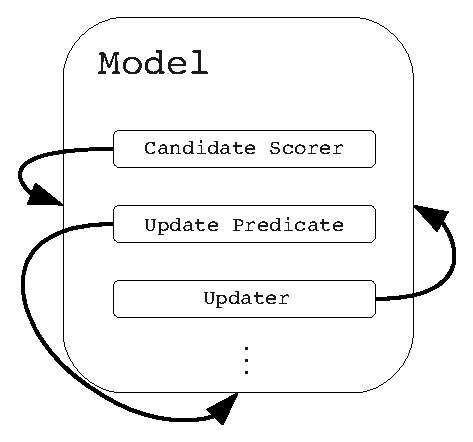
\includegraphics[bb=120bp 400bp 345bp 610bp,clip,scale=2.0]{figures/model-diagram.eps}
\end{center}

\section{Cluster-based distributed training}
\begin{itemize}
  \item ReFr seamlessly integrates with Hadoop MapReduce framework to provide distributed training of large reranking models
  \item ReFr uses iterative parameter mixtures (IPM) \cite{mcdonald10distributed}
\end{itemize}

\vspace{1cm}
\begin{center}
\hspace{-9cm} 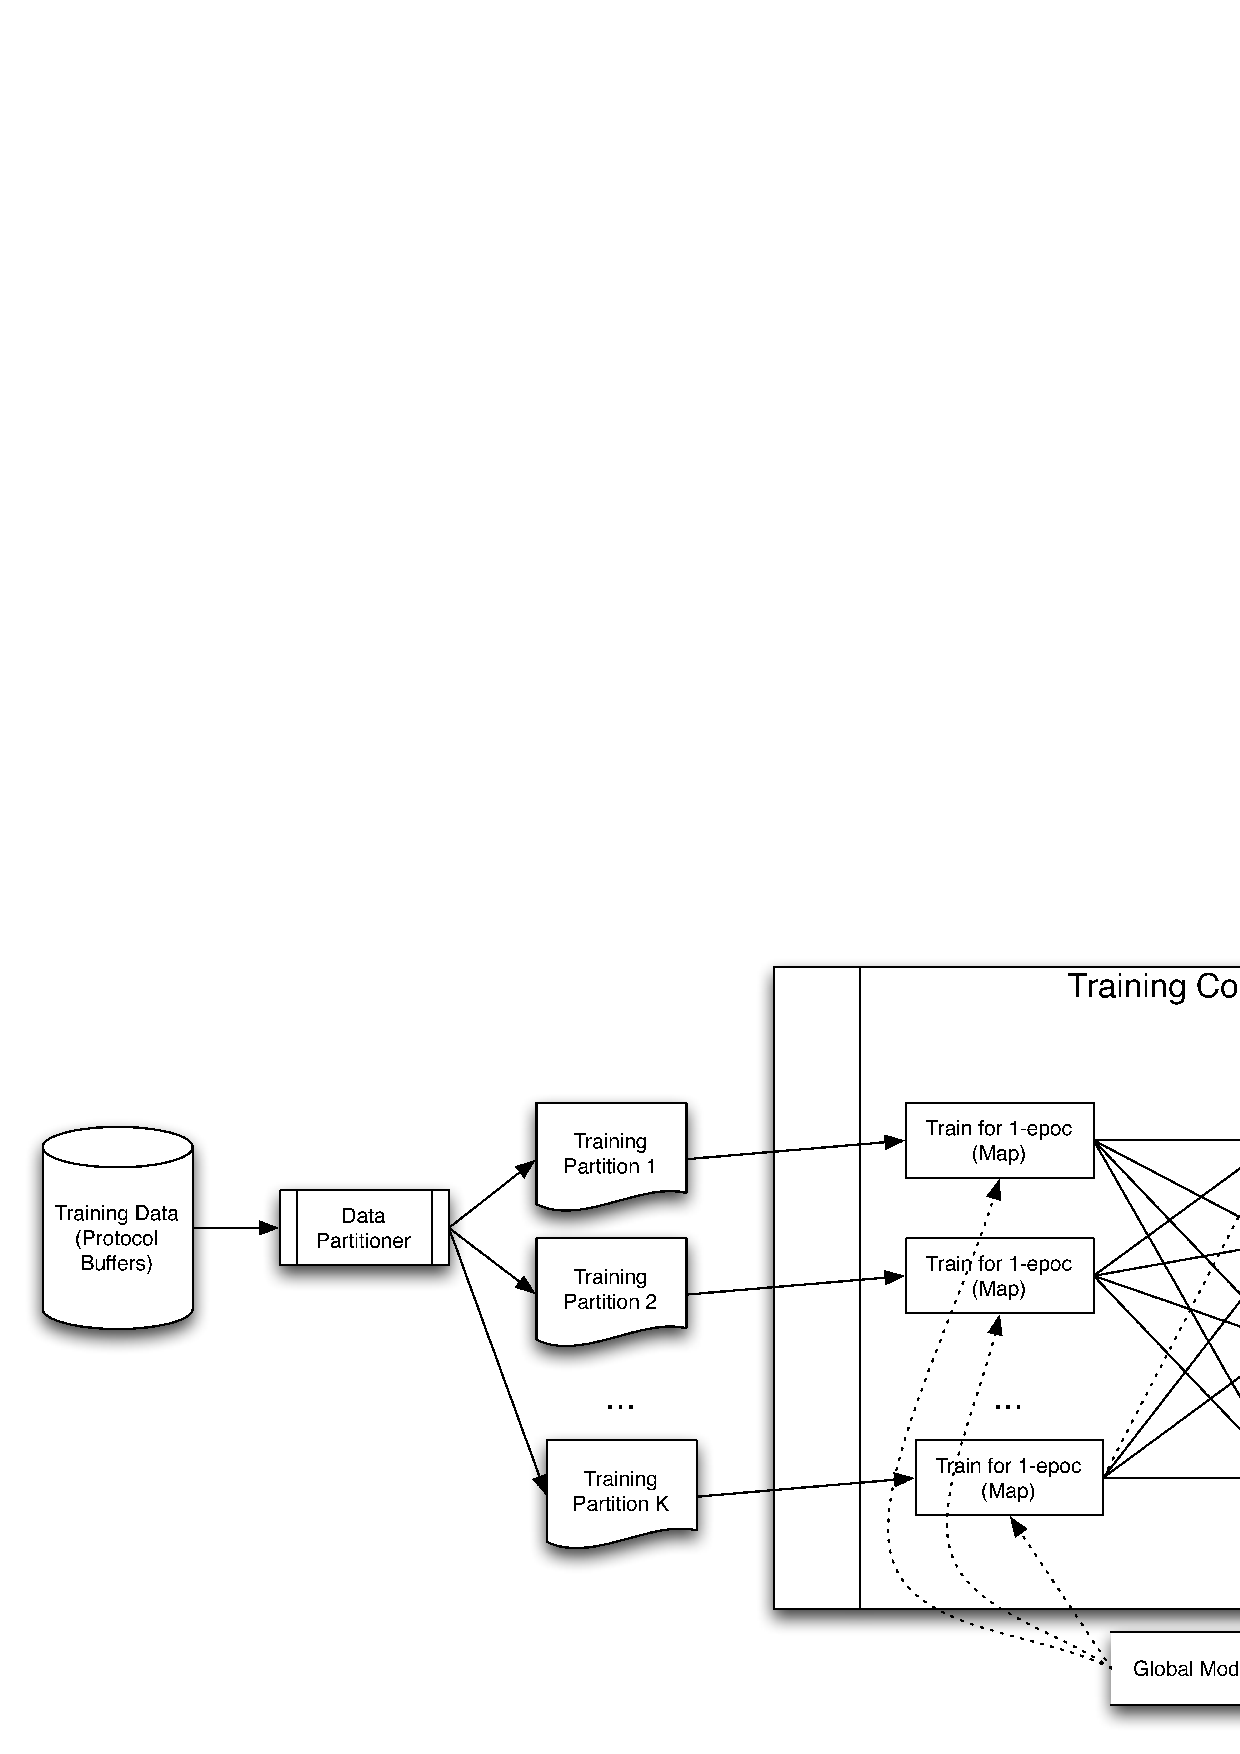
\includegraphics[scale=1.4]{figures/mapreduceflow} 
\end{center}

\section{Download and use ReFr}
\begin{itemize}
\item Available now at \texttt{http://refr.googlecode.com}
\item Only need to download and install \texttt{protobuf} package
\item (optional) Install hadoop on your cluster
\item Use ReFr and profit!
\end{itemize}

\section{The Future}
\begin{itemize}
\item New learning methods
\item More compact representation for n-gram features
\item Additional distributed training methods
\end{itemize}

\small
\bibliographystyle{IEEEtran}
\bibliography{refr}

\end{document}

\end{center}
